\chapter{Case Study: Application to MLP Conformance Testing}

\label{chapter_network_replication}

{I}{n} the design and test of control and signal processing systems, methods whereby a system under test is stimulated with a signal so that system performance parameters can be inferred from the resulting response are of fundamental importance.  For a linear system under test, such methods comprise the fundamentals of linear system identification and provide a basis for the comparison of control system performance \cite{ogata_modern_control}.  For nonlinear systems, choice of the stimulus signal and parameter identification strategy often incur system specific challenges that would need to be addressed \cite{aguirre_birds_2019}.  In this chapter, a system identification based strategy is presented for determining the weights of fundamental neural network systems and subsystems, and is applied to the conformance testing of MLP neural networks.

Inspired by multi-sinusoidal system identification techniques developed for electrical and electro-mechanical systems \cite{wambacq_distortion_1998,novak_nonlinear_2010,myslinski_large_signal_2005,schreurs_multisine_2003,schreurs_rf_2003,witters_black_box_2009}, the procedure involves stimulating a neural network or a fundamental sub-circuit inside a large network with an interrogation signal and then collecting the responses.  Then, following the methods of model stealing / replication \cite{tramer_stealing_2016,papernot_practical_2017,oh_reverse_2019,duddu_stealing_2018,orekondy_knockoff_2019}, a replicated neural network is fit to match the measured response for the given stimulus.  Because the weights of a replicated network are not guaranteed to uniquely match the original due to the existence of symmetric configurations of the same weights \cite{sussmann_uniqueness_1992,albertini_uniqueness_1993} or output-equivalent networks with different weights \cite{dimattina_how_2010}, a systematic method is introduced to check if the weights of the replicated network represent a network with behavior equivalent to the specification.  This step accepts the weights of two networks as inputs, and returns a measure of similarity indicating if the two neural networks will have approximately equivalent output.

The model replication step is used to provide the test engineer with a guarantee that the stimulus applied yields suitable coverage to achieve a comprehensive test.  If the signal does not provide sufficient test coverage, the model replication step will fail and the test will fail as a result.  A failed test is therefore indicative of (a) an insufficient test signal or (b) a network defect. Introduction of this step biases the test towards a low false negative rate of defect detection while offering the test engineer high confidence in a passing result and the opportunity to further inspect a failed result by switching to a more comprehensive test signal. This procedure is thus intended to serve as a bridge between traditional system identification, network replication, and the task of verifying that a network has been implemented to meet a specification.  The full procedure serves as a reliable \textit{conformance test}, as defined in Chapter \ref{chapter_definitions}, which can be used to guarantee that a neural network implemented as a small component of a larger hardware system matches a designed neural network, even without direct access to the latent signals and weights of the implemented network, and without reliance on the ability to measure response to test vectors perfectly.

In the following sections we begin by describing the MLP conformance testing application and
problem setup along with the use case / need for
an MLP conformance test in Section \ref{sec_application_description}.  The conformance test
method and variations thereof are then described in detail in Section \ref{section_equivalency_test_steps}.  With the conformance
test defined we apply it to two sets of subject networks for two main groups of experiments.  In experiment
group A, Section \ref{sec_small_mlp_results}, we select as the subject for testing a trivial MLP architecture
with two inputs, three hidden nodes, and one output.  A group of experiments is then conducted to demonstrate
the reliability of the conformance test.  This trivial case is used to conduct a variety of experiments with
the aim of understanding the conformance test's properties in-depth.  In Section \ref{sec_large_mlp_results},
a more realistic set of subject MLPs are used, with varying numbers of hidden neurons ranging from three to $100$
to investigate the scalability of the technique.  These networks are chosen to represent the types of networks
which could be employed in a neural control system.
The specific the method and parameters employed for experiment groups A and B are detailed respectively
in Sections \ref{sec_small_mlp_results} and \ref{sec_large_mlp_results}.

\section{Application Description and Problem Setup}
\label{sec_application_description}
As an example application, consider a neural network
used in the control of a fielded hardware system. In such
applications, it can be advantageous to rapidly develop
models via open-source software tools
\cite{scikit-learn,pytorch,tensorflow}
and then exploit the efficiency of numerous proposed
hardware approaches for implementation
\cite{misra_artificial_2010,maliuk_experimentation_2015,abdelsalam_accurate_2016,schuman_survey_2017}.
However, separating design from implementation in this manner
motivates the question: how does one confirm that the
network implemented in hardware is output-equivalent
to the network originally designed?
The answer is first complicated by equivalent
symmetric configurations of a given network
\cite{sussmann_uniqueness_1992,albertini_uniqueness_1993}
and by small perturbations in parameters
yielding approximately equivalent input-output maps
\cite{dimattina_how_2010}.
One naive solution to these challenges would be
for the test procedure to mandate disassembling the network
hardware to check each weight individually.  However, this
would be impractical for large networks and might not be
possible for networks implemented in embedded hardware.
Furthermore, even if the test engineer could extract each
weight individually, the weights implemented in hardware
might not match the specification exactly due to inevitable imprecisions.
Due to nonlinearity, it is unclear what degree of output deviation
represents a defect.  Finally, measurement noise obscures the true error
between the implemented input-output map and the original
input-output map.

The role of the AMITE polynomials in the conformance test procedure
is as follows. First, the weights of the implemented network are extracted
following the methods of model stealing / replication
\cite{tramer_stealing_2016,papernot_practical_2017,oh_reverse_2019,duddu_stealing_2018,orekondy_knockoff_2019} to fit a new model
to a set of stimulus-response pairs.  Then following the
methods of Chapter \ref{chapter_improved_expansions}
the weights are converted analytically to an AMITE polynomial
representation and compared to the AMITE
representation of the original network. Here the AMITE
coefficients provide a means to assess equivalence directly
from the replicated and original weights in a manner that satisfies the requirement
to ignore output-equivalent representations of the same network
without relying on latent signals or knowledge of true latent weights.
This is possible because output-equivalent networks will have equivalent AMITE polynomial
representations. While comparing outputs directly is prone to measurement noise
errors, comparing the polynomial representations of the identified weights
provides a means of comparing the learned functions themselves.
As noted above, the preceding replication
step is used to provide a guarantee that the stimulus applied
yields suitable coverage to achieve a comprehensive equivalency
test. If the test signal does not provide sufficient coverage
invalid weights will be extracted and the test will fail.
The observed efficacy of the equivalency test is therefore dependent on the
expansion technique's ability to effectively and efficiently
expand the entire MLP as a polynomial over a desired domain,
and thus serves as empirical validation of the expansion
technique's utility, complementing the theoretical
development in Chapter \ref{chapter_improved_expansions}.

This approach eliminates the need to test weights individually.
Instead, small networks can be conformance tested holistically as grey-boxes
and large neural networks can be tested as collections of individual
sub-circuits such as those identified in recent explainability works
\cite{karpathy_visualizing_2015,zhou_object_2015,bau_network_2017,olah2020zoom}.
The full procedure therefore enables artificial intelligence practitioners
to design a neural network in software, specify its weights and
architecture for implementation in hardware, and provide both
the hardware and specification to a third party to test for conformance.
The ability to do so without latent signal access and without sharing a common
data-set could enable effective cross-organizational collaboration and
third party testing without sharing proprietary data-sets.  A flow diagram
for a conformance test is shown in Fig. \ref{fig_dev_process}.
An example system integration process which could make use of such a
conformance test is shown in Fig. \ref{fig_neural_system_dev_process}.  Note in
Fig. \ref{fig_neural_system_dev_process} that steps in each column may
be executed by different engineers or even different organizations.
\begin{figure}[!t]
	\centering
	\textit{Network Conformance Testing}\par\medskip
	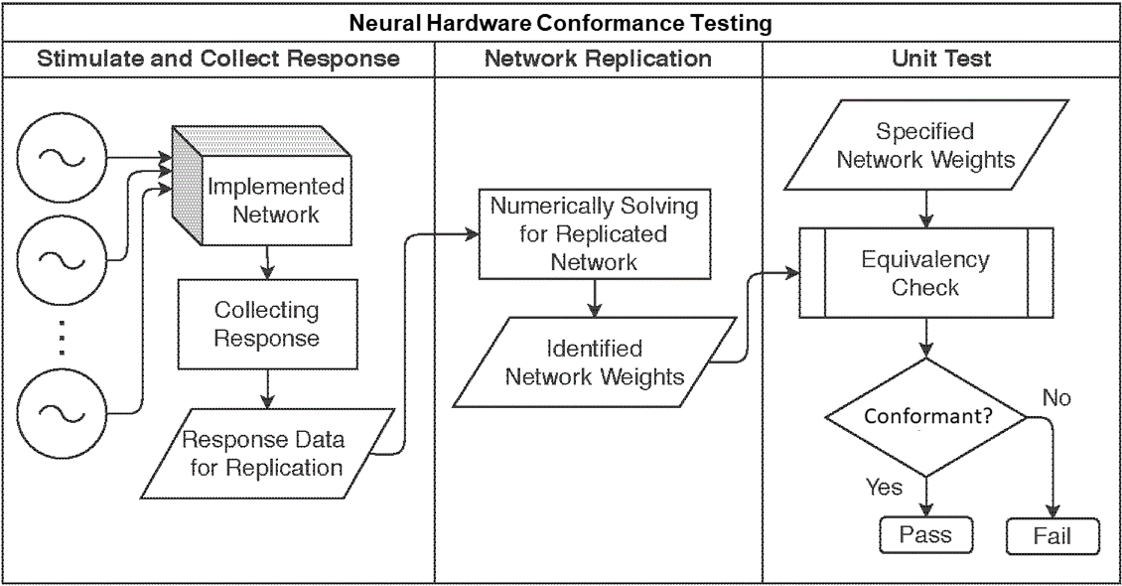
\includegraphics[width=0.8\textwidth]{Images/TestProcedure.png}
	\caption[Neural Network Conformance Test]{Conformance test procedure applying network replication to verify implemented neural network hardware or sub-circuits / sub-networks within a neural network.  An implemented network of known structure with unknown weights is stimulated by sinusoids of different frequencies and the unknown weights are identified from the response.  The identified weights are checked for equivalency to the specified weights to determine if the implemented network conforms to the original network.}
	\label{fig_dev_process}
\end{figure}
\begin{figure}[hbt!]
	\makebox[\textwidth][c]{
		
\includegraphics[width=0.8\textwidth]{images/NeuralSystemDevProcess.png}}
	\caption[Use Case for a Neural Network Conformance Test]{
		\label{fig_neural_system_dev_process} Example use case for a network conformance test showing how unit level conformance testing fits into a larger system development process before integration and system level testing. A software design firm trains a network on a proprietary data set and then provides a specification to a hardware manufacturing firm to implement the network.  The software firm then provides the specification to a third party tester who must check that the implemented network is compliant with the specification before allowing a systems integrator to integrate the network with a larger system.
	}
\end{figure}

\section{MLP Conformance Test Steps}
\label{section_equivalency_test_steps}
The specific steps of the conformance test are as
follows. First, an interrogation signal, $x_I(t)$,
is activated to stimulate the implemented network.  Several options are
available for the interrogation signal, including multi-tone sinusoidal
interrogation, noisy sinusoidal interrogation, and pure noise interrogation.
Sinusoids have the advantage of yielding a periodic response from the network
which is easy to measure in its entirety.  Since the response signal as given in Eq. 
(\ref{eq_network_output_full_expansion}) is a weighted sum of the multiples of the
components of the stimulus signal vector, it can be inferred that the fundamental
period of the response signal can be computed as the least common multiple of
the periods of the individual stimulus signals.  Measuring the response for
the duration of at least one fundamental period guarantees the full capture of the response signal.
Noise interrogation alternatively carries the benefit of high entropy coverage
of the input space but does not yield an output that is periodic or of an expected
form.  Noisy sinusoids provide a compromise between the two strategies, yielding
a higher entropy interrogation signal than pure sinusoids with an approximate fundamental
period. Noise can be injected additively, in frequency, and/or phase.  
Multiple interrogation signals can be employed sequentially and should be
chosen judiciously to match the use case.  Once the interrogation signal is applied,
the measured output along with any incurred measurement
noise $\mathcal{N}$ is collected and denoted
$\hat{y}_I(t) = y\left(\alpha, \beta_I, x_I(t)\right) + \mathcal{N}.$
The input and measurement output pairs $\left(x_I, y_M\right)$ are
then used to numerically solve for the replicated network weights
$\beta_{R}$ by fitting:
\begin{equation}
	\label{eq_optimization_for_replicated_network}
	\beta_R = \
	\underset{\beta}{\arg\min}\left(
	\left(\hat{y}_I(t) - y\left(\alpha, \beta, x_I(t)\right)\right)^2
	\right)
\end{equation}
Since the expected $\beta$ values are known in advance, they can optionally be
used as a starting point for fitting in order to significantly expedite extraction of $\beta_R$
and avoid false positives due to multiple local minima, at the expense of
some false negatives due to a test signal of insufficient coverage
still converging to the expected $\beta$.  If a compromise is required, an initial
value some distance from the expected $\beta$ may be selected instead.
The optimization problem is solved over the input vectors $x_I$.  A wide variety of
optimization methods may be employed.  In experiment group A, a trust region reflexive
optimizer is employed and in experiment group B, a stochastic gradient descent algorithm
with adaptive learning rate is employed.

The original and replicated networks are then represented analytically
via the methods of Section \ref{section_full_single_layer_expansion}
as multivariate AMITE polynomials having coefficients
$\Psi(\alpha, \beta_O) = \left[
\Psi_{\kappa_n}(\alpha, \beta_O)
\right]$ and
$\Psi(\alpha, \beta_R) = \left[
\Psi_{\kappa_n}(\alpha, \beta_R)
\right]$ respectively.  To check equivalency, a number of different
error metrics can be used.  One option is an inverse hyperbolic sine
scaled mean difference between the coefficients:
\begin{equation}
	\label{eq_error_asinh_metric}
	\eta(\Psi(\alpha, \beta_O), \Psi(\alpha, \beta_R)) =
	\mean\left(\left|\asinh\left(\frac{\Psi(\alpha, \beta_O)}{2}\right) - \asinh\left(\frac{\Psi(\alpha, \beta_R)}{2}\right)\right|\right)
\end{equation}
This error metric may be chosen to account for the large variability
in the size of the coefficients.  Larger numerical errors are less
significant for large coefficients than they would be for smaller
coefficients.  To preserve the signs of the coefficients while
achieving logarithmic-like error compression inverse hyperbolic sine scaling
can be employed. Alternatively, a mean absolute logarithmic error between the
magnitudes of the coefficients can be employed:
\begin{equation}
	\begin{split}
		\label{eq_log_error_metric}
		\eta(\Psi(\alpha, \beta_O), \Psi(\alpha, \beta_R)) =
		\mean\left|
		\log\left(\epsilon + |\Psi(\alpha, \beta_O)|\right) -
		\log\left(\epsilon + |\Psi(\alpha, \beta_R)|\right)
		\right|.
	\end{split}
\end{equation}
While the former error metric of Eq. \ref{eq_error_asinh_metric}
will detect as non-conformant  two networks with the same AMITE coefficients
but different signs, the latter metric of Eq. \ref{eq_log_error_metric} will
treat them as the same network.  Meanwhile,
the former error metric is less sensitive to small changes in small
coefficients than the latter.  The right error metric must therefore
be chosen judiciously for the application. In either case, if the
error $\eta$ is below a set threshold $\varepsilon$ the
networks are determined to be equivalent.
In the following sections, inverse hyperbolic sine scaling is employed
for all experiments in group A and logarithmic scaling is employed
for all experiments in group B.  The large size of the networks in
experiment group B tend to make individual defects less impactful to the
network's output manifold and the sensitivity of logarithmic
scaling is therefore required to achieve a reliable test.

\section{Experiment Group A: Small MLPs}
\label{sec_small_mlp_results}
\subsection{Method and Experiment Setup}
In this experiment group, small MLPs having two inputs, three hidden neurons, and one output
are considered.
We computationally model the process of stimulating the network under test, collecting the responses with measurement noise (modeled as white Gaussian), identifying a replicated network, and checking the replicated network for compliance.  We determine the optimal error threshold $\varepsilon$ by varying $\varepsilon$ for a population of 150 defective and 150 compliant networks and recording the true and false positive rates of defect detection (Fig. \ref{fig_dev_process}) with respect to $\varepsilon$.  We then instantiate a group of 100 networks and introduce defects into 50 of them.  We run the procedure of Fig. \ref{fig_dev_process} on each network and track how many of the defects were identified.  We repeat the process with increasing amounts of measurement noise and observe the effects on defect identification statistics.

Sinusoidal stimulus signals are employed since the small network size reduces the need for the very high entropy of a noise interrogation signal. Of the individual frequencies selected for the components of the test signal vector, we desire a combination that provides (1) good coverage of the network's output surface and (2) yields a response signal with a short fundamental period thus resulting in a quick but comprehensive capture of the output surface for the network under test, realizing the benefits of the sinusoidal input. We use Shannon entropy as a measure of the coverage provided by a stimulus signal.  We compute the Shannon entropy of a given stimulus signal by considering the signal sampled in discrete time well above the Nyquist rate, and then treating each combination of discrete values as a symbol $\varsigma_i$.  The entropy $\mathrm{H}$ of the stimulus signal $x$ is therefore given by $\mathrm{H}(x) = - \sum_i P(\varsigma_i) \log P(\varsigma_i)$.  As is well known in the analysis of nonlinear circuits \cite{wambacq_distortion_1998}, stimulus signals with components having frequencies that are integer multiples of other components do not provide sufficient coverage to serve as test signals.

An example signal that provides good entropy without yielding a large fundamental period is:
\begin{equation}
	x = \begin{pmatrix}
		\sin(5t) \\
		\sin(4t)
	\end{pmatrix}
	\label{eq_stimulus_5_4}
\end{equation}
An example signal that provides better entropy at the cost of a larger fundamental period is:
\begin{equation}
	x = \begin{pmatrix}
		\sin(11t) \\
		\sin(10t)
	\end{pmatrix}
	\label{eq_stimulus_11_10}
\end{equation}\
Our observations of the reliability of the verification procedure are shown with respect to stimulus signal choice in Fig. \ref{fig_accuracy_wrt_entropy}.

Once the response to the stimulus signal is measured, the next step is to solve for the weights $\beta_R$ of a replicated network.  This is achieved through numerically solving Eq. (\ref{eq_optimization_for_replicated_network}).  We apply a trust region reflective algorithm to find $\beta_R$ for this group of experiments.
For the final step of determining if the replicated network $\beta_R$ is output-equivalent to the original network $\beta_O$ we compare the $\Psi$ coefficients of each network $\Psi(\alpha, \beta_O)$ and $\Psi(\alpha, \beta_R)$.  We compute these coefficients according to the algorithm of Fig. \ref{fig_generate_psi}.  Applying the error metric of Eq. (\ref{eq_error_asinh_metric}), we determine if the error between $\Psi(\alpha, \beta_O)$ and $\Psi(\alpha, \beta_R)$ is greater than an acceptable tolerance $\varepsilon$.  Based on our observations in tuning $\varepsilon$ shown in Fig. \ref{fig_roc_curve}, we choose $\varepsilon = 1$ as our tolerance to use in the collection of experimental results for this experiment group.

\subsection{Results}
\subsubsection{Stimulus and Response Signals}
The example stimulus signal $x$ of Eq. (\ref{eq_stimulus_5_4}) is shown in Fig. \ref{fig_stimulus_54} along with the resulting response $y(\alpha, \beta, x)$ for a randomly selected small network under test with two inputs, three hidden neurons, and a single output.  The same stimulus signal's coverage of the circuit's output contours is shown in Fig. \ref{fig_stimulus_with_output_contours}.  The output of the same small neural circuit is shown with respect to its input components $x_1$ and $x_2$.  The path that the stimulus signal takes across the output contours is shown.
\begin{figure}[!htp]
	\centering
	\textit{Stimulus and Response Signals}\par\medskip
	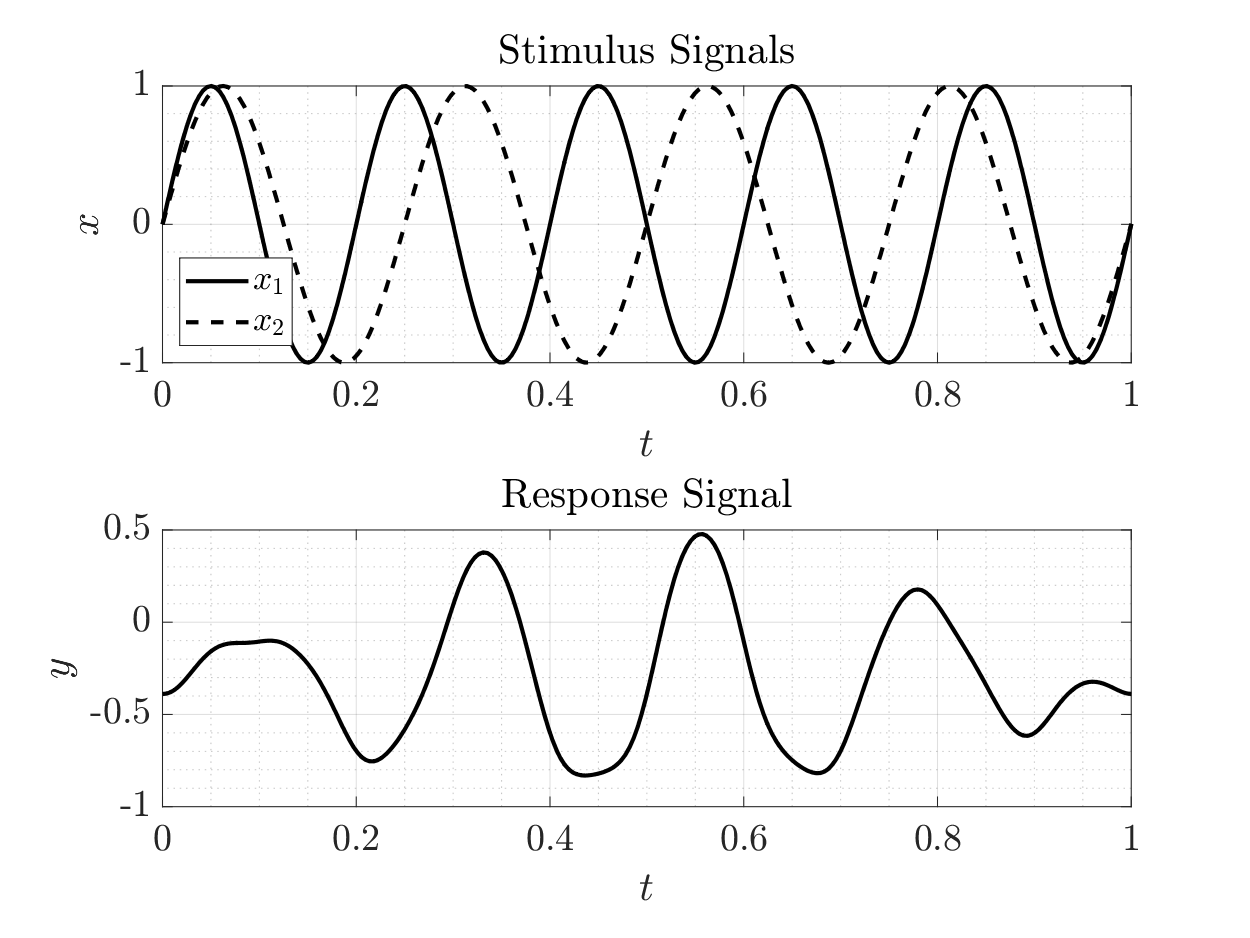
\includegraphics[width=0.7\textwidth]{Images/ExampleStimulusAndResponse.png}
	\caption[Example Stimulus Signals]{An example stimulus signal and its resulting response signal are shown.  The stimulus signal has two components: $x_1(t) = \sin(5t)$ and $x_2(t) = \sin(4t)$. The resulting response shown is the output of a random network under test under application of this stimulus signal.}
	\label{fig_stimulus_54}
\end{figure}
\begin{figure}[!hbp]
	\centering
	\textit{Stimulus Signal and Network Output Contours}\par
	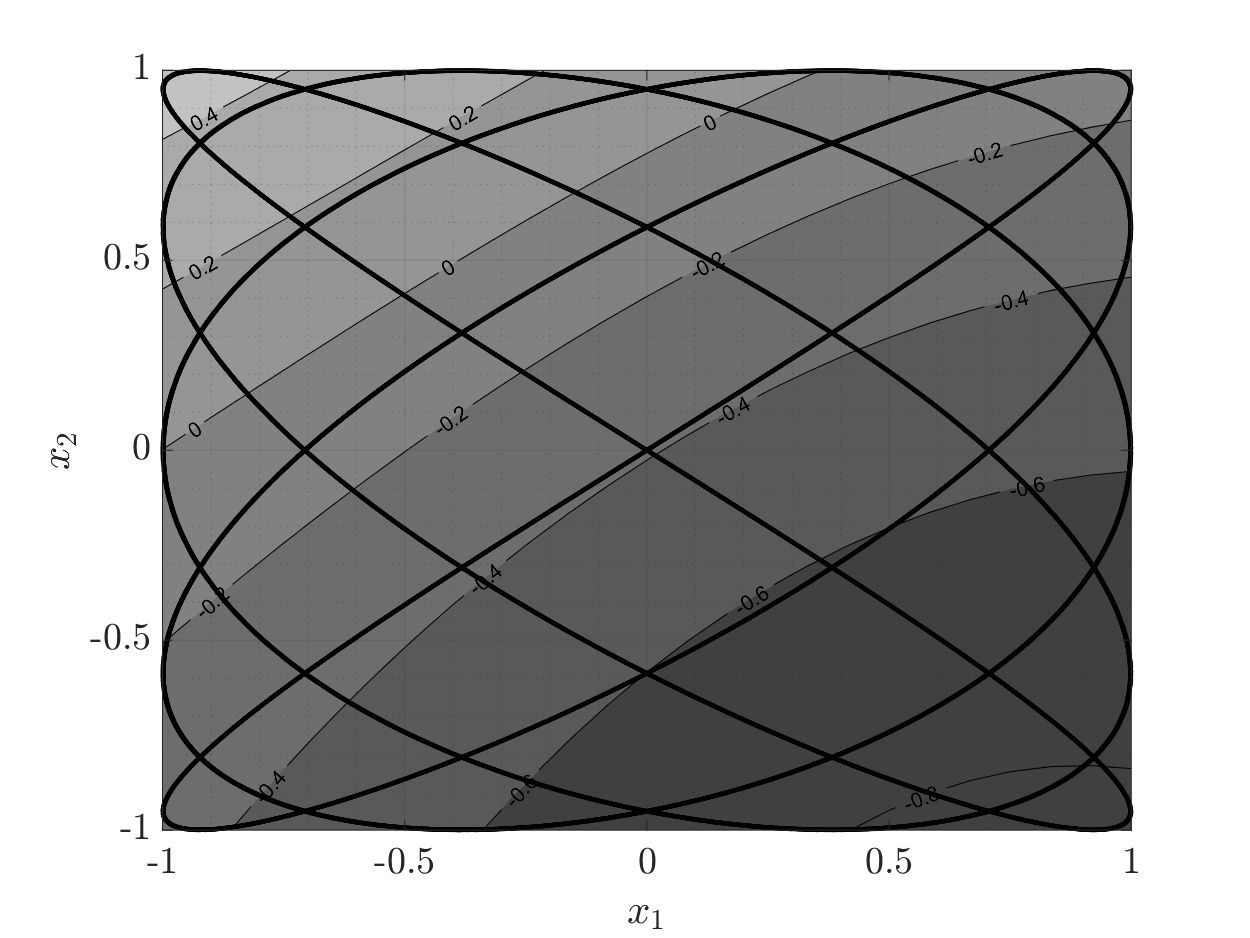
\includegraphics[width=0.65\textwidth]{Images/ExampleStimulusCoverageBW_54.png}
	\caption[Stimulus Signal and Network Output Contours]{The path that an example stimulus signal follows over the contours of a random network under test is shown as a black line.  The output of the network over any $(x_1, x_2)$ pair is shown as a contoured surface.  The stimulus signal has two components: $x_1(t) = \sin(5t)$ and $x_2(t) = \sin(4t)$.}
	\label{fig_stimulus_with_output_contours}
\end{figure}
To assess the effect of the stimulus choice on the accuracy of the verification procedure, we execute the verification procedure of Fig. \ref{fig_dev_process} over a population of 100 networks, where 50 have randomly introduced defects.  Each network represents a small neural circuit having two inputs, three hidden neurons, and one output.  We repeat the verification procedure using stimulus signals having several $(\omega_1, \omega_2)$ pairs and observe how many of the defects are correctly identified to compute the accuracy of the procedure for each stimulus signal.  The entire experiment is repeated 10 times using different random measurement noise and introducing new random defects each round.  In this experiment, defects are created by introducing random changes to the weights of the network under test.  We observe that non-integer ratios between selected stimulus signal frequencies provide higher signal entropy and that higher entropy stimulus signals result in more reliable detection of the defective networks.
\begin{figure}[!b]
	\centering
	\textit{Effect of Stimulus Signal Choice
		on Accuracy of Defect Detection Procedure}\par\medskip
	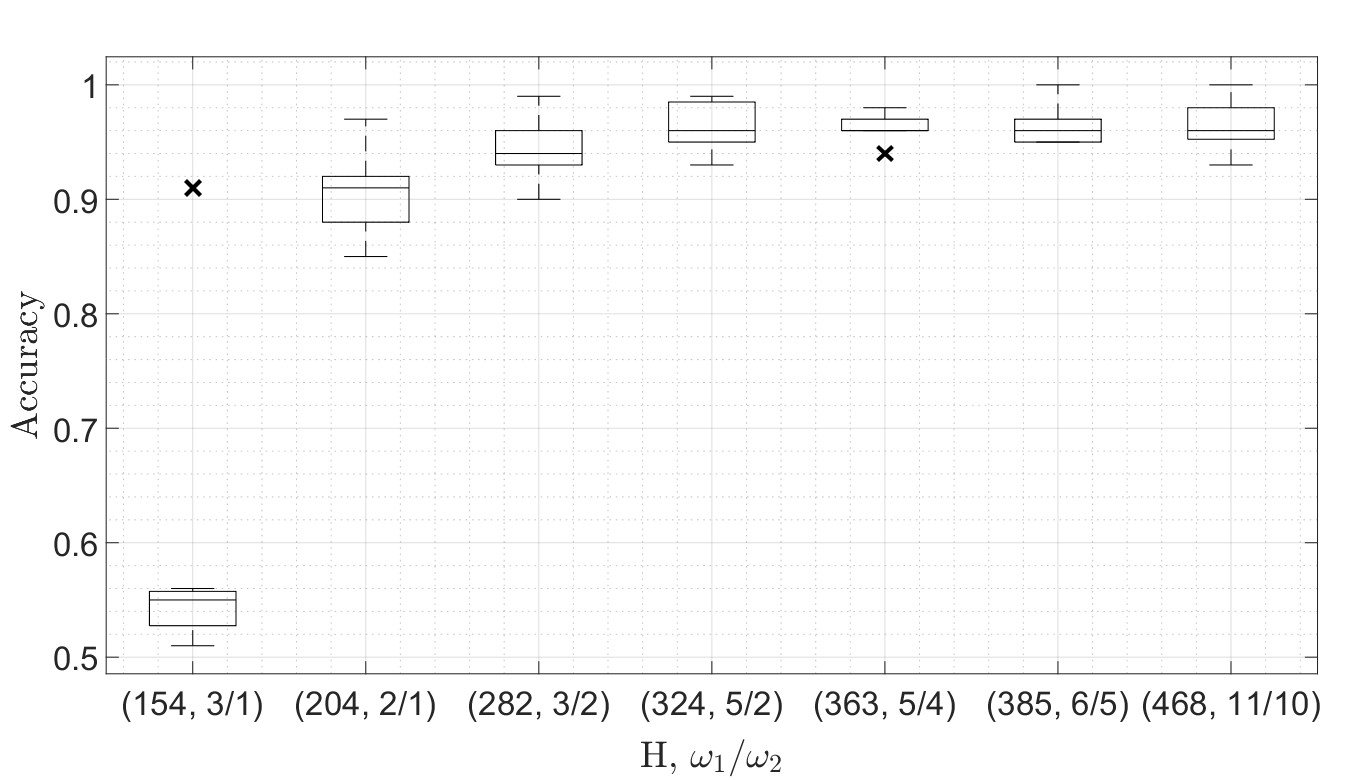
\includegraphics[width=0.95\textwidth]{Images/AccuracyWrtEntropyCropped.png}
	\caption[Defect Detection Accuracy]{Defect detection accuracy is shown for several stimulus signals.  Accuracy statistics were computed over a population of 50 defective networks and 50 compliant networks. The verification procedure was run on each network with a measurement SNR of 100 dB, and the experiment was repeated using several stimulus signals 10 rounds each using different random noise each round.  Stimulus signal entropy $\mathrm{H}$ is shown along with the frequency ratio of the stimulus signal components $\frac{\omega_1}{\omega_2}$.  We observe that non-integer ratios between $\omega_1$ and $\omega_2$ provide higher entropy and a more reliable test.}
	\label{fig_accuracy_wrt_entropy}
\end{figure}

\subsubsection{Testing the Conformance Test}
To determine if checking the error between the $\Psi$ coefficients using the error metric of Eq. (\ref{eq_error_asinh_metric}) is a valid means to assess the conformance of different sets of original and replicated network weights, we conduct four experiments, where different kinds of output-equivalent and non-output-equivalent networks are compared.
\begin{enumerate}
	\item In an \emph{exactly conformant networks} experiment we instantiate two copies of the same network and demonstrate that the error metric $\eta(\Psi(\alpha, \beta_1), \Psi(\alpha, \beta_2))$ of Eq. (\ref{eq_error_asinh_metric}) is zero for $\beta_1 = \beta_2$.
	\item In a \emph{symmetrically conformant networks} experiment we instantiate two networks with weights rearranged in obviously symmetric configurations such as those discussed by Sussmann \cite{sussmann_uniqueness_1992} and Albertini \cite{albertini_uniqueness_1993}.  We demonstrate that the error metric $\eta$ is still zero for these symmetric configurations.
	\item In a \emph{approximately conformant networks} experiment we instantiate two copies of the same network and introduce in one network a small perturbation in the hidden layer weights (i.e., after the nonlinear activation) to cause a proportionally small change in the input-output relationship.  We  demonstrate that in this case $\eta$ is non-zero but still small (i.e., $0<\eta<1$), as is the desired behavior.
	\item In a \emph{nonconformant networks} experiment we instantiate two completely different networks and demonstrate that $\eta$ is large (i.e., $\eta>1$), as is the desired behavior.
\end{enumerate}

In each experiment, a two input, three hidden neuron, single output circuit with random weights is used as a test case. The results of the symmetrically conformant networks test, the approximately conformant networks test, and the non-conformant networks test are shown in Fig. \ref{fig_sym_equiv_test}, \ref{fig_approx_equiv_test}, and \ref{fig_non_equiv_test} respectively.
\begin{figure}[!t]
	\centering
	\textit{Symmetrically Conformant Networks Comparison}\par\medskip
	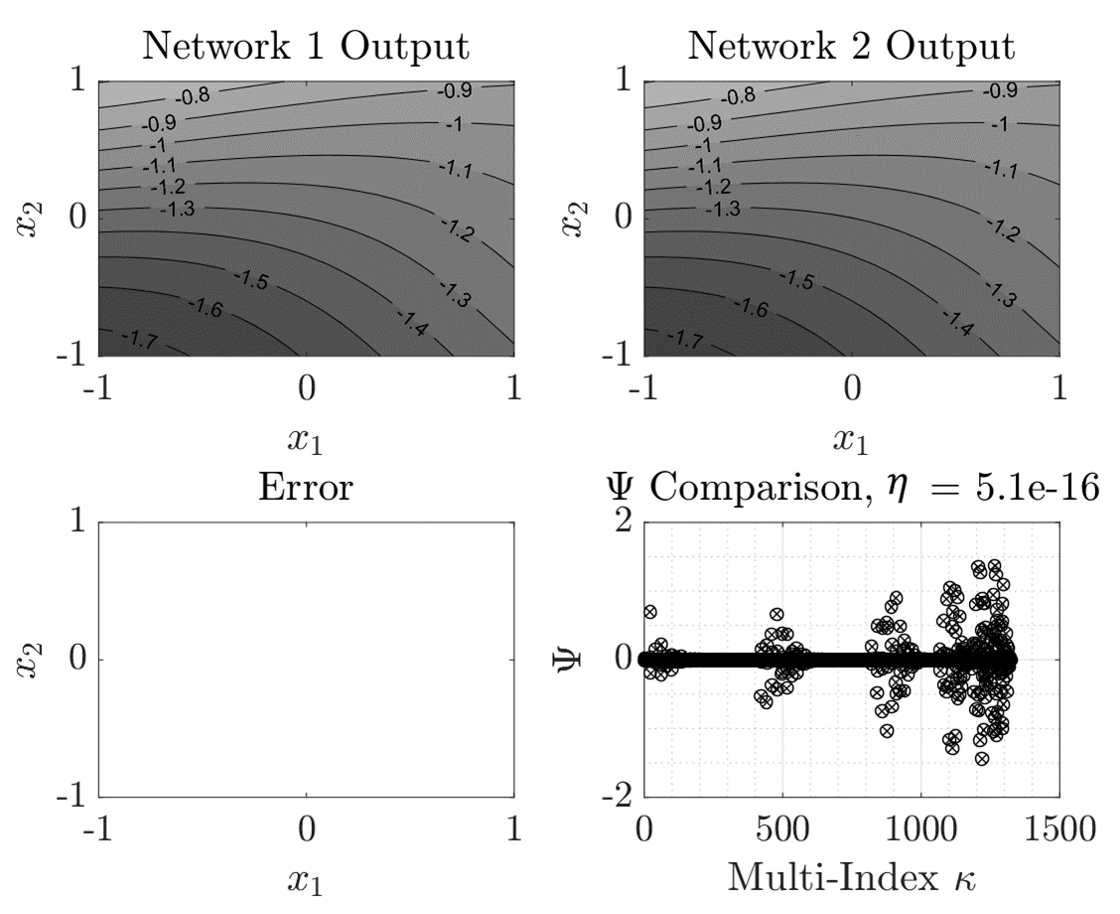
\includegraphics[width=0.9\textwidth]{Images/2DClassificationContourCoverageBWSymEqualCropped.png}
	\caption[Symmetrically Conformant Networks Comparison]{Output contours over a 2D input space are shown for two symmetrically Conformant neural networks.  The symmetrically conformant networks were generated by creating two exactly conformant networks and exchanging neurons in one of the networks to create a network with the same behavior as the first but with a different configuration of the same weights.  The $\Psi_\kappa(\alpha, \beta_1)$ and $\Psi_\kappa(\alpha, \beta_2)$ coefficients match exactly as is expected behavior.}
	\label{fig_sym_equiv_test}
\end{figure}
\begin{figure}[!t]
	\centering
	\textit{Approximately Conformant Networks Comparison}\par\medskip
	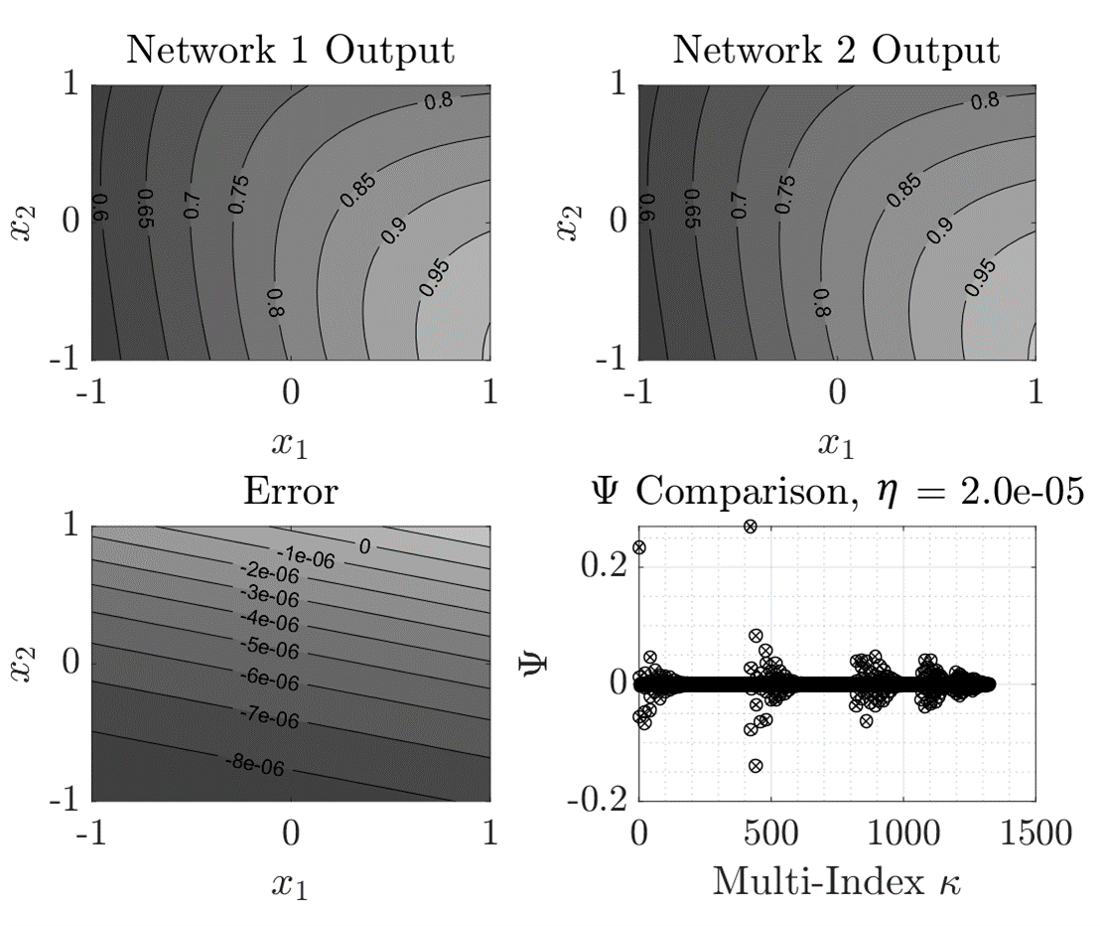
\includegraphics[width=0.9\textwidth]{Images/2DClassificationContourCoverageBWApproxEqualCropped.png}
	\caption[Approximately Conformant Networks Comparison]{Output contours over a 2D input space are shown for two approximately conformant neural networks.  The approximately conformant networks were generated by creating two exactly conformant networks and introducing into one of the networks a small error that does not noticeably affect performance and therefore does not represent a defect.  The $\Psi_\kappa(\beta_1)$ and $\Psi_\kappa(\beta_2)$ coefficients match closely as is expected, yielding an error metric $\eta(\Psi(\beta_1), \Psi(\beta_2)) < 1.0$.}
	\label{fig_approx_equiv_test}
\end{figure}

\begin{figure}[!t]
	\centering
	\textit{Non-Conformant Networks Comparison}\par\medskip
	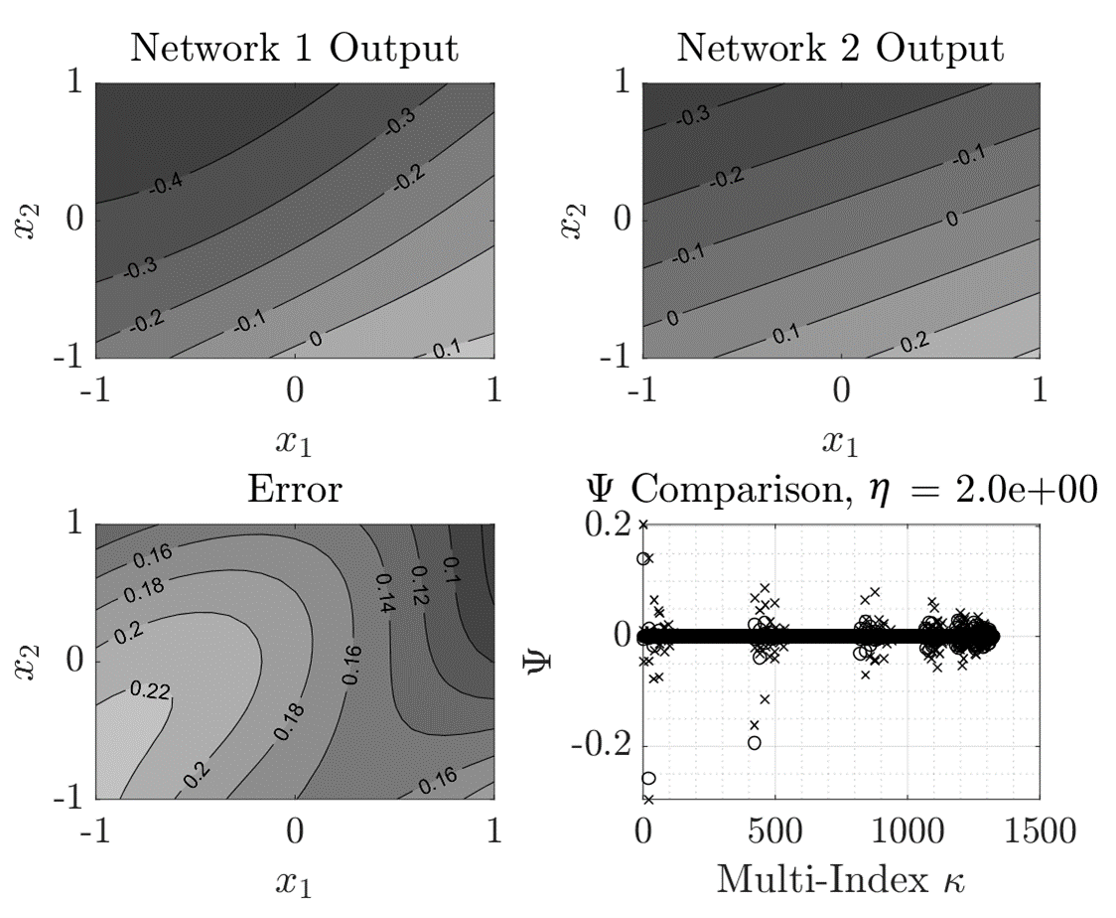
\includegraphics[width=0.9\textwidth]{Images/2DClassificationContourCoverageBWNotEqualCropped.png}
	\caption[Non-Conformant Networks Comparison]{Output contours over a 2D input space are shown for two non-conformant neural networks.  The two non-conformant networks were generated by randomly perturbing the weights of two exactly conformant networks.  The $\Psi_\kappa(\alpha, \beta_1)$ and $\Psi_\kappa(\alpha, \beta_2)$ coefficients do not match and yield an error metric $\eta(\Psi(\alpha, \beta_1), \Psi(\alpha, \beta_2)) > 1.0$ as is expected.}
	\label{fig_non_equiv_test}
\end{figure}

\subsubsection{Conformance Testing a Population of Networks}

To confirm that $\eta < \varepsilon,\ \varepsilon = 1$ is a valid condition for determining conformant networks, we perform a test where the error threshold is swept and the accuracy of the procedure of Fig. \ref{fig_dev_process} is recorded with respect to the threshold.  A population of 300 small neural circuits is instantiated, each having two inputs, three hidden neurons, and one output.  These networks under test could represent a small standalone nonlinear circuit or small components of a larger neural network being analyzed.  We select 150 of the 300 small networks under test and introduce defects into them by adding random perturbations to the existing weights.  The correct weights are saved off as the specified network weights.  We run the defect detection procedure using different error tolerances spanning from $\varepsilon=10^{-6}$ to $\varepsilon=10^{2}$ and track the true positive and false positive rates of the test, where a true positive is a correctly identified defect and a false positive is an incorrectly identified defect.  The error tolerance sweep is repeated with signal to measurement noise ratios of $25\mathrm{dB}$, $50\mathrm{dB}$, and $100\mathrm{dB}$.

\begin{figure}[!t]
	\centering
	\textit{Defect Detection True and False Positive Rates with Respect to Error Tolerance $\varepsilon$}\par\medskip
	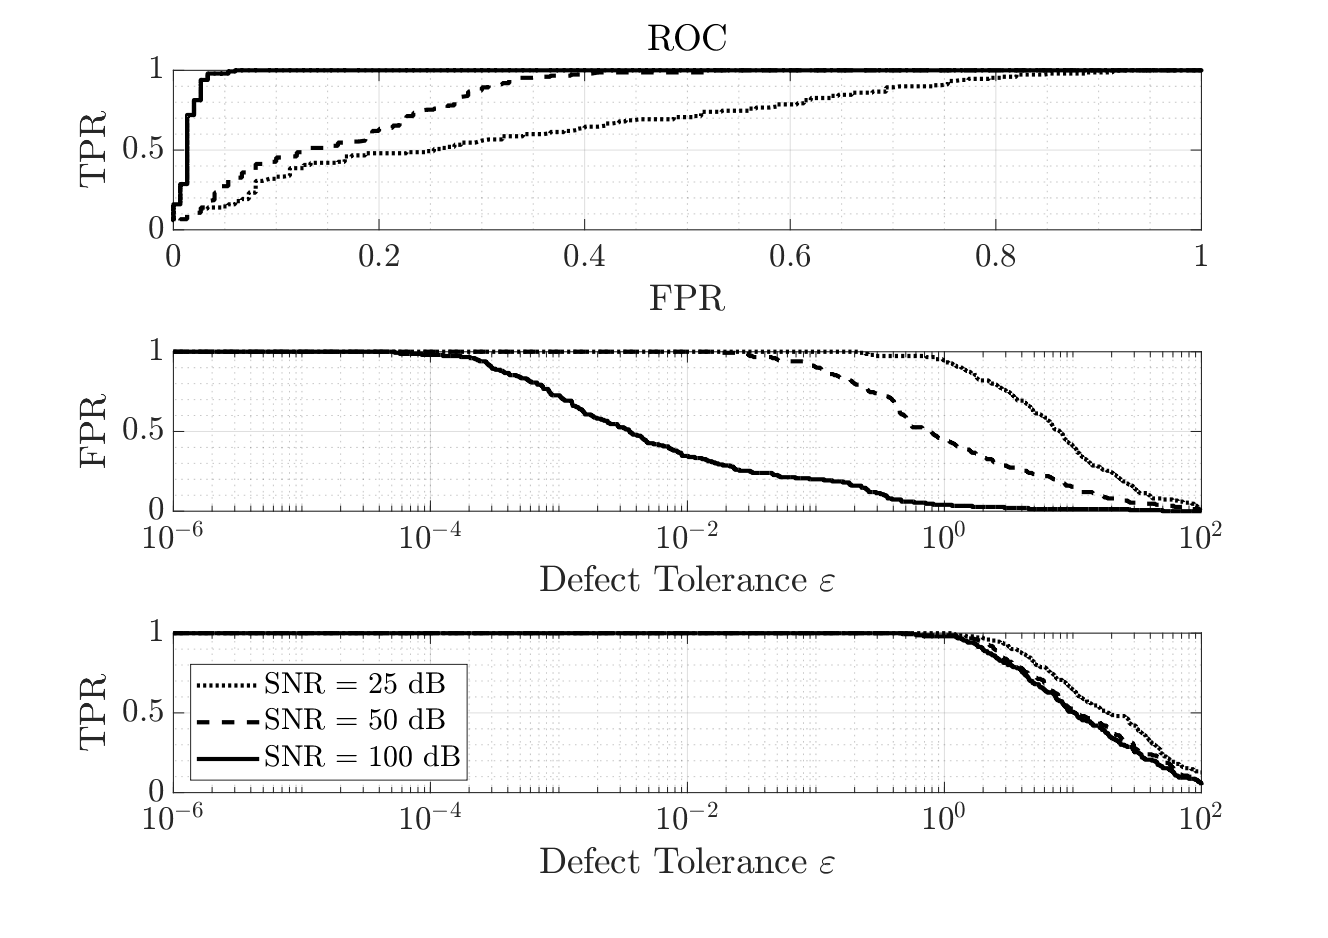
\includegraphics[width=0.95\textwidth]{Images/ROCcropped.png}
	\caption[Defect Detection True and False Positive Rates with Respect to Error Tolerance]{Receiver Operating Characteristic curves are shown for the verification procedure. A population of 150 defective networks and 150 compliant networks were used to generate the curves.  The $\Psi_\kappa(\beta)$ coefficients were computed for all networks and the verification procedure was executed with different defect tolerances $\varepsilon$.  The entire experiment was repeated using different signal to noise ratios.}
	\label{fig_roc_curve}
\end{figure}

We find that $\varepsilon = 1$ provides a suitable balance between low false positive rates and high true positive rates.  False and true positive rates are shown in Fig. \ref{fig_roc_curve}.  We observe that false positives are caused by the optimizer failing to replicate the network under test in the time allowed (we limit the number of function evaluations to 10K, and limit the number initial seeds the solver is allowed to try to 20 to keep run times consistent).  A false positive could be rectified by allowing the optimizer to run longer on potentially defective networks under test.

\begin{figure}[!t]
	\centering
	\textit{Defect Detection Accuracy wrt. Measurment Noise Ratio - Experiment A}\par\medskip
	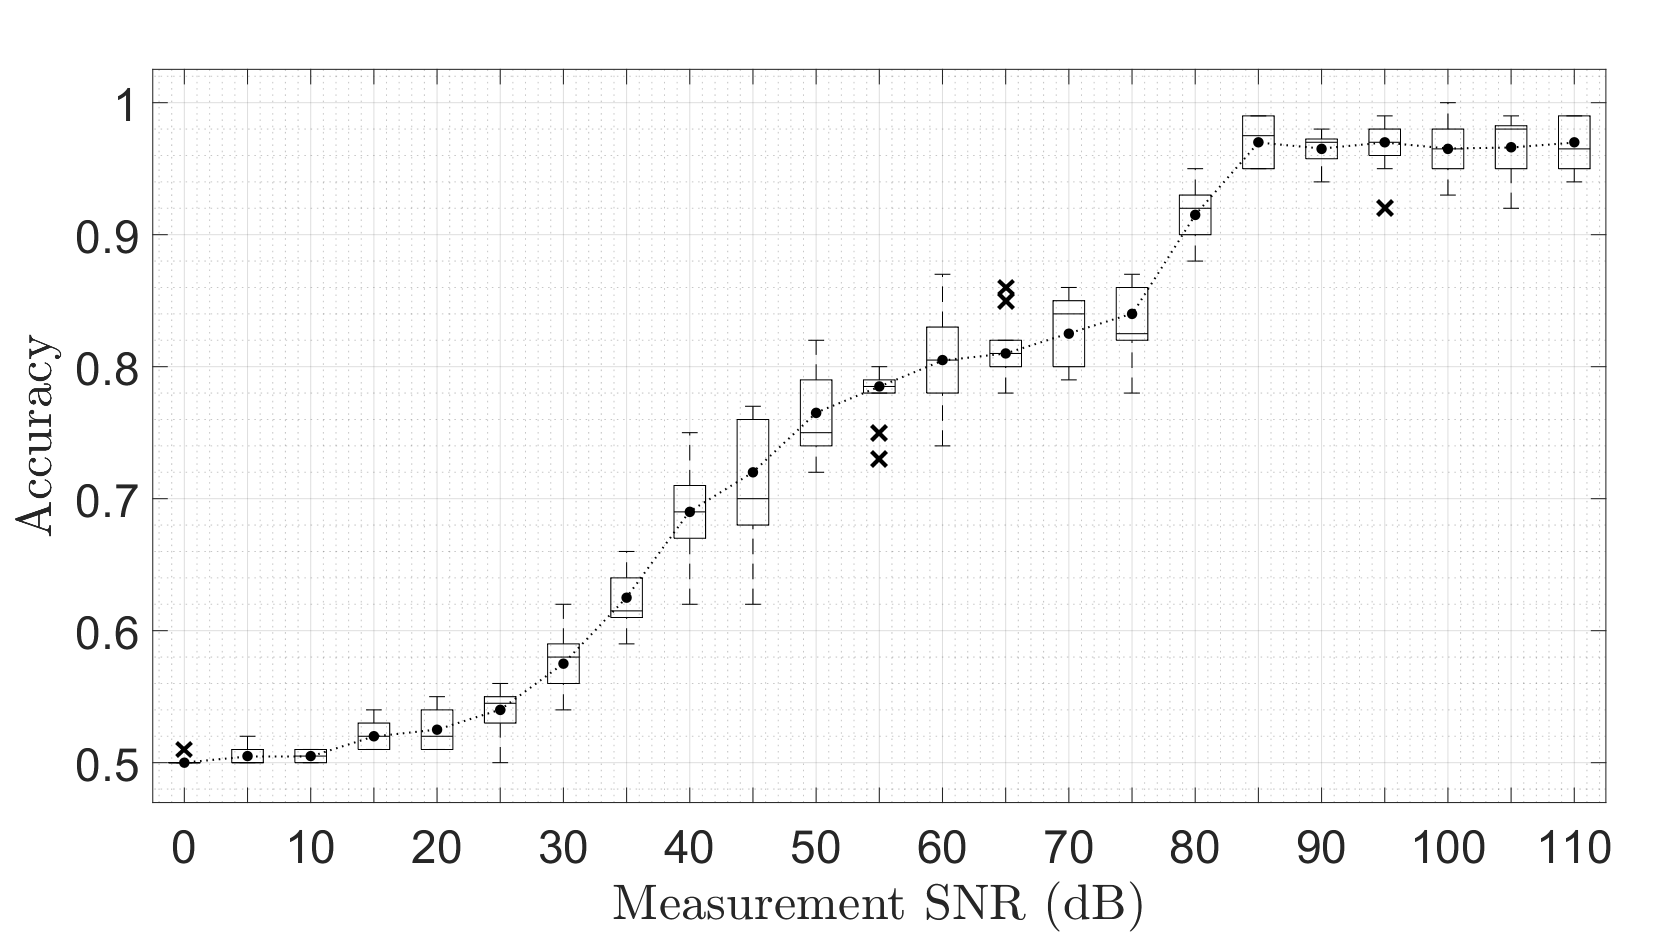
\includegraphics[width=0.8\textwidth]{Images/AccuracyWrtSNRCropped.png}
	\caption[Defect Detection Accuracy wrt. Signal to Noise Ratio]{Defect detection accuracy with respect to signal to measurement noise ratio is shown.  Accuracy statistics were computed over a population of 50 defective networks and 50 compliant networks. The verification procedure was run on each network for each measurement SNR shown.  The entire experiment was repeated 10 times for each SNR with different random measurement noise for a total of 23000 calls to the test procedure.  Mean and median accuracy are shown as black dots and black lines respectively.}
	\label{fig_accuracy_wrt_snr}
\end{figure}

With a suitable tolerance for identification of non-conformant networks determined, we create a population of 100 networks, where 50 are compliant with the corresponding specified network and 50 have defects.  We run the defect detection procedure of Fig. \ref{fig_dev_process} on all 100 networks for measurement signal to noise ratios between $0\mathrm{dB}$ and $110\mathrm{dB}$ and observe the accuracy of the defect identification procedure.  We repeat the entire procedure 10 times with different random defects and different random noise. Observed test procedure accuracy with respect to measurement SNR is summarized in Fig. \ref{fig_accuracy_wrt_snr}.

\section{Experiment Group B: Larger MLPs}
\label{sec_large_mlp_results}

\subsection{Method and Experiment Setup}
In this experiment group, MLPs having two inputs, many hidden neurons,
and one output are considered to assess scalability.
The experimental process for experiment group B for was modeled computationally on a
Dell XPS Laptop and parallel processing was used to achieve the timing results reported.
All computations were implemented in Python 3.7
using the pytorch, numpy, cupy, and mpmath libraries on an
Nvidia GeForce GTX 1650 GPU with 1024 Cuda Cores and an
Intel i9-9980HK CPU running at 2.40GHz.  Parallel processing
was implemented through standard pytorch and cupy matrix operations.
Coefficients for $\tanh$ and ReLU were precomputed using 450 digits
of precision via the precise formulas of Chapter \ref{chapter_improved_expansions}
and polynomials were evaluated at runtime in IEEE 754 double precision floating
point arithmetic.  General mathematical primitives including
binomial and multinomial coefficients were precomputed and stored
in hashmaps for fast access at runtime.  Multinomial coefficient
hashmaps required 4.73GB of disk space and were loaded into
program memory as needed in chunks ranging from 11KB to 986MB
for fast access.

To collect results for the method of section
\ref{section_equivalency_test_steps} on larger MLPs, a population of 90 MLPs
is instantiated having inputs $N_I \in \{1, 2, 3\}$ and number of hidden nodes
$N_H \in \{5, 10, 35, 75, 125\}$.  The population is then duplicated to
model a set of networks under test.  Defects in the form of random
weight perturbations are then introduced into half of the population
of networks under test. The network conformance test of
Fig. \ref{fig_dev_process} is executed following the methods
of Section \ref{section_equivalency_test_steps} on each network.  All 90
networks are tested with different levels of noise
$\mathcal{N} \in \{-20, -10, -1, 0, 1, 10, 20\}\ \mathrm{dB}$.  The entire procedure is
repeated three times for a total of 1890 calls to the conformance test.
The accuracy of the conformance test at finding bugs is reported in 
Fig. \ref{fig_accuracy_wrt_snr} with respect to signal to noise
ratio in the measured outputs of the network under test.  Runtime with
respected to number of hidden nodes and number of inputs is reported in
Fig. \ref{fig_runtime_wrt_hidden_units} and
\ref{fig_runtime_wrt_num_inputs} respectively.  For all
tests an error threshold of $\varepsilon = 0.01$ was applied
when checking conformance by the logarithmic error metric of
Eq. (\ref{eq_log_error_metric}):
$
\eta(\Psi(\alpha, \beta_O), \Psi(\alpha, \beta_R)) > \varepsilon
$.  We find that the test completes in under 7 seconds on average
for low-dimensional input (2-4 inputs) MLPs having up to 125
hidden nodes.  The runtime per test is inclusive of both solving
for the replicated network parameters and computing the AMITE
polynomial representation.

\subsection{Results}
The results for experiment group B are summarized in Figures
\ref{fig_accuracy_wrt_snr2}, \ref{fig_runtime_wrt_hidden_units}, and
\ref{fig_runtime_wrt_num_inputs}.  Figure \ref{fig_accuracy_wrt_snr2}
shows the results of a measurement noise sweep for the population of
larger networks.  We observe enhanced noise robustness in this group of
experiments, which can be attributed to the high entropy interrogation signals
employed, sensitive error metric of Eq. \ref{eq_log_error_metric}, use
of the expected $\beta_R$ as a seed for the optimization, and through the use
of regularized stochastic gradient descent with adaptive learning rate to
replicate the network.  Overall, these improvements introduced in experiment group B
yield a more robust test.  Figure \ref{fig_runtime_wrt_hidden_units} summarizes
runtime with respect to number of hidden units and Figure \ref{fig_runtime_wrt_num_inputs}
summarizes runtime with respect to number of inputs for the population of larger
networks.  As would be expected from the form of the algorithm in Section
\ref{section_full_single_layer_expansion}, runtime scales linearly with respect to the number of hidden
units but scales with factorial growth with respect to the number of inputs.  We therefore conclude
that the technique can be easily scaled to many hidden neurons, but is only of practical
utility for networks with a small number of inputs, such as those which would be used in
neural control applications where the inputs are a small number of states, in contrast to
image classifiers, for example, where the inputs are a large number of pixels.
\begin{figure}[!t]
	\centering
	\textit{Defect Detection Accuracy wrt. Measurment Noise Ratio - Experiment B}\par\medskip
	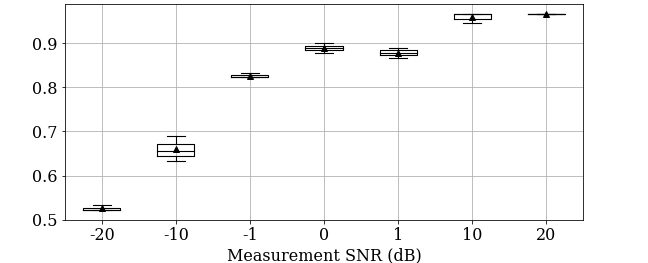
\includegraphics[width=0.95\textwidth]{Images/accuracy_male_wrt_snr.png}
	\caption[Bug Detection Accuracy with Respect to Measurement Noise]{Bug detection accuracy with respect to measurement noise.
		Shows the fraction of defective networks under test which were
		correctly identified.  Results are aggregated over 1890 calls
		to the conformance test on networks of varying sizes under
		various levels of noise.
	}
	\label{fig_accuracy_wrt_snr2}
\end{figure}
\begin{figure}[ht!]
	\centering
	\textit{Runtime (s) wrt. Number of Hidden Units, ($N_H$)}\par\medskip
	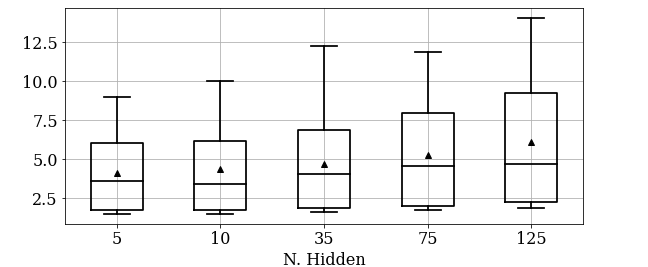
\includegraphics[width=0.9\textwidth]{Images/runtime_wrt_n_hidden.png}
	\caption[Runtime per Call With Respect to Number of Hidden Units]{Runtime per call to the test with respect to number of
		hidden units, $N_H$.  Statistics are computed across 1890 calls to the
		test.
	}
	\label{fig_runtime_wrt_hidden_units}
\end{figure}
\begin{figure}[ht!]
	\centering
	\textit{Runtime (s) wrt. Number of Inputs, ($N_I$)}\par\medskip
	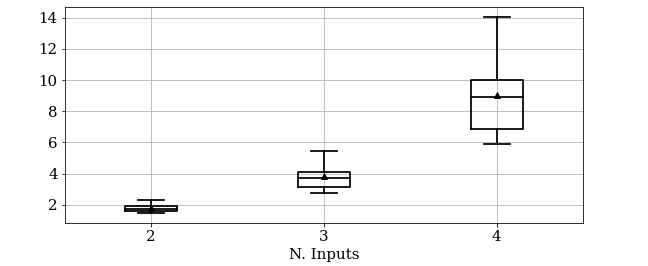
\includegraphics[width=0.95\textwidth]{Images/runtime_wrt_num_inputs.png}
	\caption[Runtime per Call With Respect to Number of Inputs]{Runtime per call to the test with respect to number of
		inputs, $N_I$. Statistics are computed across 1890 calls to the
		test.
	}
	\label{fig_runtime_wrt_num_inputs}
\end{figure}
